%%%%%%%%%%%%%%%%%%%%%%%%%%%%%%%%%%%%%%%%%%%%%%%%%%%%%
%                                                   %
%     Penn State Colloquium Poster Template         %
%                                                   %
% Uses Penn State Colloquium class, with options:   %
%                                                   %
% Orientation:                                      %
%     portrait (default), landscape                 %
%                                                   %
% Paper size:                                       %
%     a4paper (default), a0paper, a1paper, a2paper, %
%     a3paper, a5paper, a6paper                     %
%%%%%%%%%%%%%%%%%%%%%%%%%%%%%%%%%%%%%%%%%%%%%%%%%%%%%
\documentclass{../psuposter}
\renewcommand{\templateimagepath}{../} 


%%%%%%%%%%%%%%%%%%%%%%%%%%%%%%%%%%%%%%%%%%%%%%%%%%%%%
%               Package Dependencies                %
%%%%%%%%%%%%%%%%%%%%%%%%%%%%%%%%%%%%%%%%%%%%%%%%%%%%%
\usepackage{natbib}
\usepackage{lipsum}                                % Dummy text
\usepackage[figwidth = 0.98\linewidth]{todonotes}  % Dummy image (and more!)
\usepackage[absolute, overlay]{textpos}            % Figure placement
\usepackage{braket}
\setlength{\TPHorizModule}{\paperwidth}
\setlength{\TPVertModule}{\paperheight}
\setcitestyle{numbers,square}


%%%%%%%%%%%%%%%%%%%%%%%%%%%%%%%%%%%%%%%%%%%%%%%%%%%%%
%                 AUTHOR AND TITLE                  %
%%%%%%%%%%%%%%%%%%%%%%%%%%%%%%%%%%%%%%%%%%%%%%%%%%%%%
\title{Departments That Excel in Equity, Diversity, and Inclusion at Penn State and Across the Nation}
\author{Edmund Bertschinger}
\institute{Massachusetts Institute of Technology}


%%%%%%%%%%%%%%%%%%%%%%%%%%%%%%%%%%%%%%%%%%%%%%%%%%%%%
%                  BEGIN DOCUMENT                   %
%%%%%%%%%%%%%%%%%%%%%%%%%%%%%%%%%%%%%%%%%%%%%%%%%%%%%
\begin{document}
\begin{frame}
\begin{columns}[t, totalwidth=\textwidth]
\begin{column}{0.45\textwidth - 1cm}


%%%%%%%%%%%%%%%%%%%%%%%%%%%%%%%%%%%%%%%%%%%%%%%%%%%%%
%                 BLOCK: BIOGRAPHY                  %
%%%%%%%%%%%%%%%%%%%%%%%%%%%%%%%%%%%%%%%%%%%%%%%%%%%%%
    \begin{block}{Speaker Biographic Summary}
    	\begin{center}
    		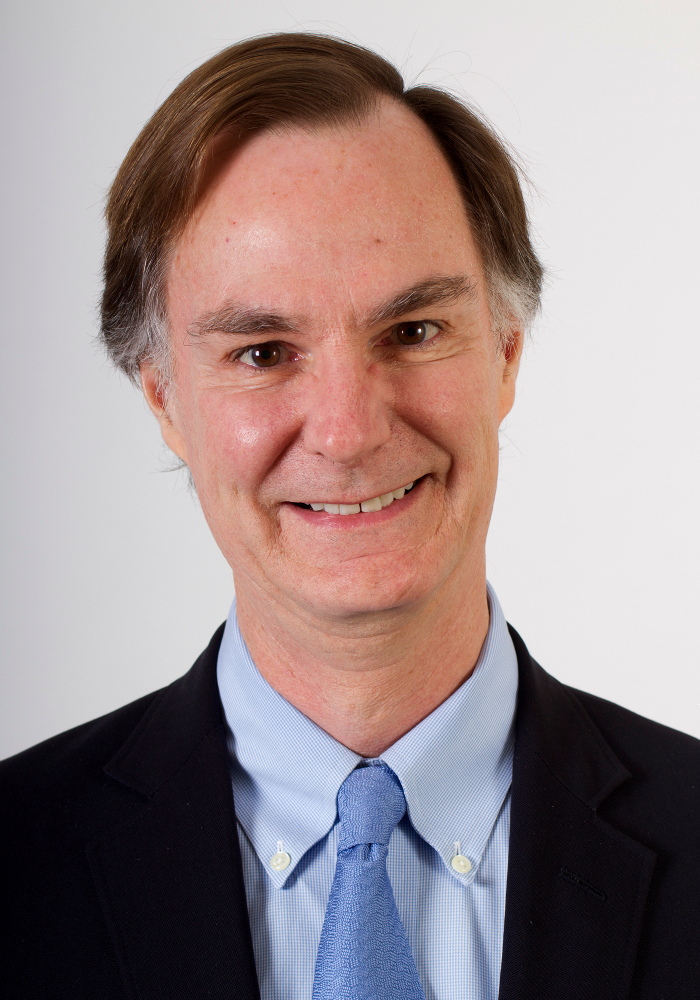
\includegraphics[width=0.68\textwidth]{images/portrait}
    	\end{center}
    	\href{https://web.mit.edu/physics/people/faculty/bertschinger_edmund.html}{Dr. Edmund Bertschinger} is a Professor of Physics at MIT with an affiliation in the MIT Program in Women’s and Gender Studies. He is a scholar-activist-administrator for diversity, equity, and inclusion in higher education. Ed served as MIT’s inaugural Community and Equity Officer from 2013–2018 and has served on numerous national committees and task forces on equity in physics and astronomy. During 2007–2013 he was Physics Department Head at MIT. He is a Fellow of both the APS and the AAAS and has won the MIT MLK Leadership Award, the Outstanding Freshman Advisor Award, a Guggenheim Fellowship, and many other awards.
    \end{block}


%%%%%%%%%%%%%%%%%%%%%%%%%%%%%%%%%%%%%%%%%%%%%%%%%%%%%
%            BLOCK: RESEARCH INTERESTS              %
%%%%%%%%%%%%%%%%%%%%%%%%%%%%%%%%%%%%%%%%%%%%%%%%%%%%%
    \begin{block}{Research Interests}
        Prof. Bertschinger's lies in theoretical cosmology, gravitation, and numerical methods, and whose passion lies in shifting the culture of STEM fields to be inclusive and equitable for everyone. His research group at MIT aims to develop and apply analytical, computational, and statistical methods to improve our understanding of the physical universe.  
        \begin{center}
	    	
\includegraphics[width=0.55\textwidth]{images/research}    		
	    	
	    	\textit{Quintessence field evolution with potential.}
    	\end{center}
    	%\cite{longResearchLongLab}
    \end{block}
\end{column}
\begin{column}{0.55\textwidth - 1cm}


%%%%%%%%%%%%%%%%%%%%%%%%%%%%%%%%%%%%%%%%%%%%%%%%%%%%%
%                 BLOCK: ABSTRACT                   %
%%%%%%%%%%%%%%%%%%%%%%%%%%%%%%%%%%%%%%%%%%%%%%%%%%%%%
    \begin{block}{Talk Abstract}
    	Women and people of color are severely underrepresented in many STEM departments, especially in physical sciences and engineering. In addition, people with intersecting marginalized identities, including sexual and gender minorities and people with disabilities, often experience unsupportive environments. Professional societies and universities have issued reports full of recommendations for improvements, but change is slow and difficult.

        In some fields and at some times, Penn State has been a leader in equity and diversity efforts. Demographic data tell a story, and the stories of individuals provide additional important data. In this talk I will present such data over nearly 60 years with the goal of helping departments in physics and other STEM disciplines create environments where all people can thrive.
    \end{block}


%%%%%%%%%%%%%%%%%%%%%%%%%%%%%%%%%%%%%%%%%%%%%%%%%%%%%
%                BLOCK: BACKGROUND                  %
%%%%%%%%%%%%%%%%%%%%%%%%%%%%%%%%%%%%%%%%%%%%%%%%%%%%%
    \begin{block}{Brief Background}
    	Prof. Bertschinger was the first person to serve as the Institute Community and Equity Officer (ICEO) at MIT, a position which was founded in 2013. \cite{EdmundBertschingerAppointed} The role of ICEO was created to build mutual understanding across the MIT community and to sustain their shared focus on increasing equity and inclusion. \cite{InstituteCommunityEquity}    
        \begin{center}
		   	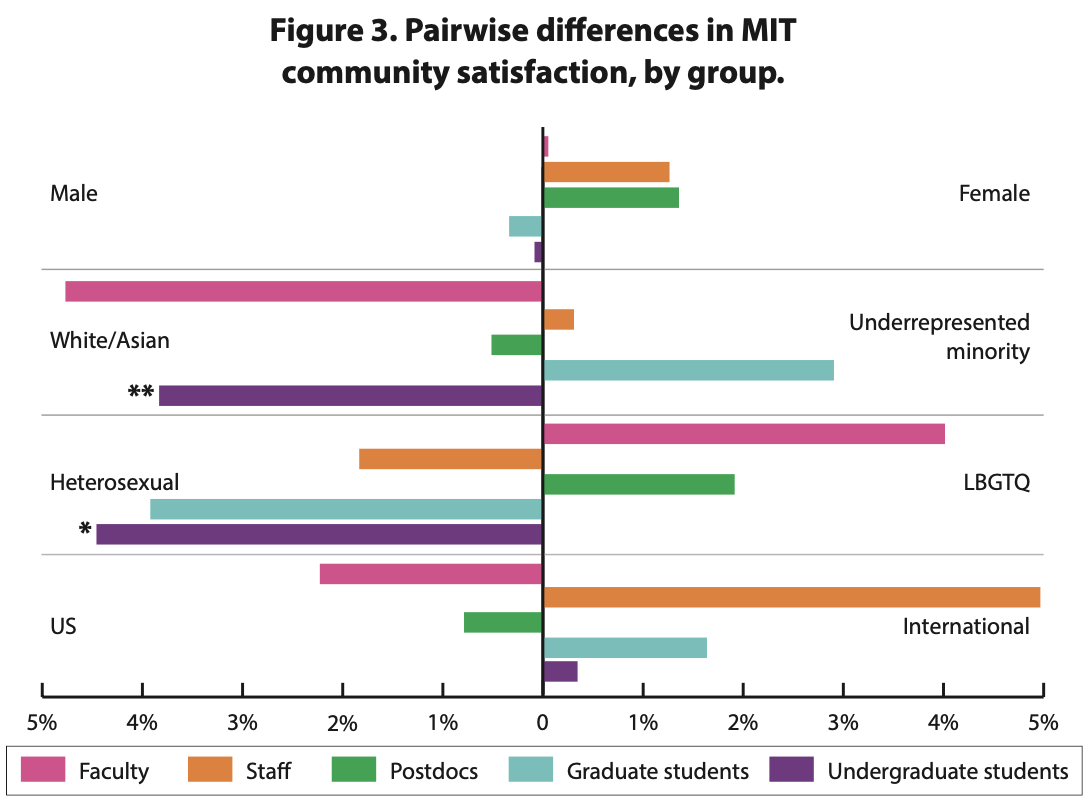
\includegraphics[width=0.65\textwidth]{images/background} 
		   	
		   	\textit{Pairwise differences in MIT community satisfaction, by group.}\cite{bertschingerAdvancingRespectfulCaring2015}
    	\end{center}
		
		Notably, Prof. Bertschinger drove the development and release of a 2015 report evaluating inclusion issues at MIT in a broad context, including the nature of everyday interactions on campus as well as diversity questions in faculty hiring. The report presciently observed that until an institution ``can embrace [its] diversity, exercise empathy, and advance caring and respect, [it] will never achieve [its] full potential.'' \cite{bertschingerAdvancingRespectfulCaring2015} 
    \end{block}


%%%%%%%%%%%%%%%%%%%%%%%%%%%%%%%%%%%%%%%%%%%%%%%%%%%%%
%                 BLOCK: REFERENCES                 %
%%%%%%%%%%%%%%%%%%%%%%%%%%%%%%%%%%%%%%%%%%%%%%%%%%%%%
    \begin{block}{References}
        \bibliographystyle{aipnum4-1}
%        \bibliographystyle{iopart-num}
		\bibliography{references}
    \end{block}

\end{column}
\end{columns}


%%%%%%%%%%%%%%%%%%%%%%%%%%%%%%%%%%%%%%%%%%%%%%%%%%%%%
%                    FOOTER TEXT                    %
%%%%%%%%%%%%%%%%%%%%%%%%%%%%%%%%%%%%%%%%%%%%%%%%%%%%%
\begin{textblock}{0.5}(0.18, 0.94)
    \color{white}
    \sffamily
    \textbf{Eberly College of Science}
    \\
    Department of Physics
\end{textblock}


%%%%%%%%%%%%%%%%%%%%%%%%%%%%%%%%%%%%%%%%%%%%%%%%%%%%%
%                   END TEMPLATE                    %
%%%%%%%%%%%%%%%%%%%%%%%%%%%%%%%%%%%%%%%%%%%%%%%%%%%%%
\end{frame}
\end{document}
